\documentclass{standalone}
\usepackage{tikz} 
\usepackage{epsf,graphicx,subfig}
\usepackage{color}
\usepackage{amssymb,amsmath}
\usepackage{scalefnt}
\usetikzlibrary{positioning}
%include other needed packages here   
\begin{document}

\begin{tikzpicture}

\definecolor{lungColor}{rgb}{0.2353, 0.6078, 0.8235}
\definecolor{chestWallColor}{rgb}{0.5294, 0.7843, 0.6078}
\definecolor{ribColor}{rgb}{0.0000, 0.4510, 0.1961}
\definecolor{pectoralColor}{rgb}{0.6510, 0.3490, 1.0000}
\definecolor{fibroGlandColor}{rgb}{1.0000, 1.0000, 0.0000}
\definecolor{fatColor}{rgb}{0.9804, 0.5882, 0.1176}
\definecolor{skinColor}{rgb}{0.9804, 0.7255, 0.7451}
\definecolor{unkTissueColor}{rgb}{0.6000, 0.3020, 0.2510}
\definecolor{bgColor}{rgb}{0.0000, 0.0000, 0.0000}
\definecolor{lesionColor}{rgb}{1.0000, 0.2510, 0.0000}
\definecolor{boundaryColor}{rgb}{0.8784, 0.8784, 0.7529}


\tikzset{nameSt/.style=
{anchor=north west,rectangle,
node distance=60.7pt,
minimum width=5pt,minimum height=5pt,
}}



\node[anchor=south west,inner sep=0] (imgNode) at (0,0) {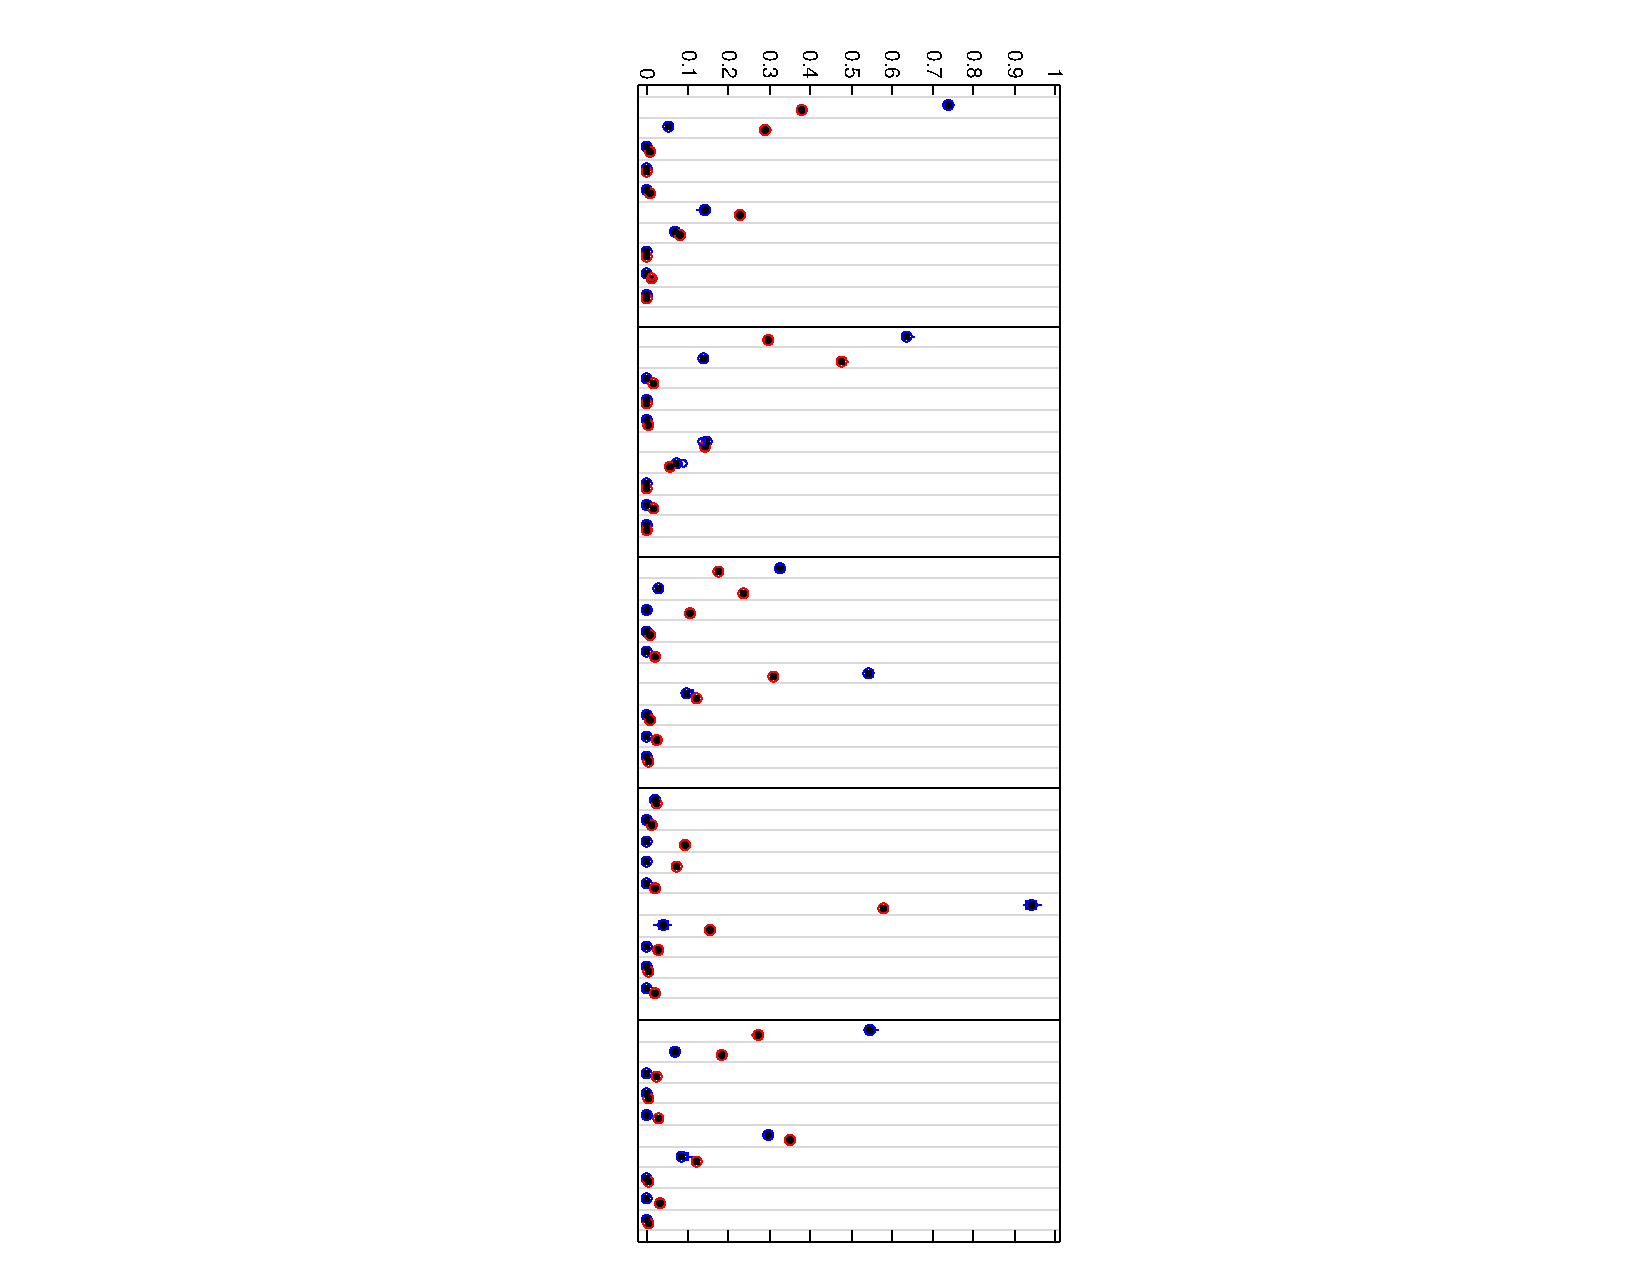
\includegraphics[trim = 305 14 277 20, clip,angle=90,width=\textwidth]{cooccurrenceMatrixA.pdf}};

\begin{tiny}

\draw[] (imgNode.north west) +(18pt,4pt) node[nameSt, draw=bgColor, fill=bgColor,label=right:Background] (bgName) {} ;
\draw[] (imgNode.north east) +(2.2,0) node[nameSt,draw=lungColor, fill=lungColor,right=of bgName,label=right:Air or lungs] (lungName) {};
\draw[] (0,0) node[nameSt, draw=chestWallColor,right=of lungName, fill=chestWallColor,label=right:Chest wall] (cwName) {} ;
\draw[] node[nameSt, draw=ribColor, fill=ribColor,right=of cwName,label=right:Rib] (ribName) {} ;
\draw[] node[nameSt, draw=pectoralColor, fill=pectoralColor,right=of ribName,label=right:Pectoral muscle] (pectoralName) {} ;

\tikzset{labelSt/.style=
{anchor=north west,rectangle,
node distance=2.6pt,
scale=.7,
minimum width=1pt,minimum height=1pt,
}}


\draw[] (imgNode.south west) +(17pt,0) node[labelSt, draw=bgColor, fill=bgColor] (bgName) {} ;
\draw[] node[labelSt,draw=lungColor, fill=lungColor,right=of bgName] (lungName) {};
\draw[] node[labelSt, draw=chestWallColor,right=of lungName, fill=chestWallColor] (cwName) {} ;
\draw[] node[labelSt, draw=ribColor, fill=ribColor,right=of cwName] (ribName) {} ;
\draw[] node[labelSt, draw=pectoralColor, fill=pectoralColor,right=of ribName] (pectoralName) {} ;
\draw[] node[labelSt, draw=fibroGlandColor, fill=fibroGlandColor,right=of pectoralName] (fibroGlandName) {} ;
\draw[] node[labelSt, draw=fatColor, fill=fatColor,right=of fibroGlandName] (fatName) {} ;
\draw[] node[labelSt, draw=skinColor, fill=skinColor,right=of fatName] (skinName) {} ;
\draw[] node[labelSt, draw=lesionColor, fill=lesionColor,right=of skinName] (lesionName) {} ;
\draw[] node[labelSt, draw=boundaryColor, fill=boundaryColor,right=of lesionName] (boundaryName) {} ;


\draw[] (imgNode.south west) +(83pt,0) node[labelSt, draw=bgColor, fill=bgColor] (bgName) {} ;
\draw[] node[labelSt,draw=lungColor, fill=lungColor,right=of bgName] (lungName) {};
\draw[] node[labelSt, draw=chestWallColor,right=of lungName, fill=chestWallColor] (cwName) {} ;
\draw[] node[labelSt, draw=ribColor, fill=ribColor,right=of cwName] (ribName) {} ;
\draw[] node[labelSt, draw=pectoralColor, fill=pectoralColor,right=of ribName] (pectoralName) {} ;
\draw[] node[labelSt, draw=fibroGlandColor, fill=fibroGlandColor,right=of pectoralName] (fibroGlandName) {} ;
\draw[] node[labelSt, draw=fatColor, fill=fatColor,right=of fibroGlandName] (fatName) {} ;
\draw[] node[labelSt, draw=skinColor, fill=skinColor,right=of fatName] (skinName) {} ;
\draw[] node[labelSt, draw=lesionColor, fill=lesionColor,right=of skinName] (lesionName) {} ;
\draw[] node[labelSt, draw=boundaryColor, fill=boundaryColor,right=of lesionName] (boundaryName) {} ;

\draw[] (imgNode.south west) +(149pt,0) node[labelSt, draw=bgColor, fill=bgColor] (bgName) {} ;
\draw[] node[labelSt,draw=lungColor, fill=lungColor,right=of bgName] (lungName) {};
\draw[] node[labelSt, draw=chestWallColor,right=of lungName, fill=chestWallColor] (cwName) {} ;
\draw[] node[labelSt, draw=ribColor, fill=ribColor,right=of cwName] (ribName) {} ;
\draw[] node[labelSt, draw=pectoralColor, fill=pectoralColor,right=of ribName] (pectoralName) {} ;
\draw[] node[labelSt, draw=fibroGlandColor, fill=fibroGlandColor,right=of pectoralName] (fibroGlandName) {} ;
\draw[] node[labelSt, draw=fatColor, fill=fatColor,right=of fibroGlandName] (fatName) {} ;
\draw[] node[labelSt, draw=skinColor, fill=skinColor,right=of fatName] (skinName) {} ;
\draw[] node[labelSt, draw=lesionColor, fill=lesionColor,right=of skinName] (lesionName) {} ;
\draw[] node[labelSt, draw=boundaryColor, fill=boundaryColor,right=of lesionName] (boundaryName) {} ;

\draw[] (imgNode.south west) +(215.5pt,0) node[labelSt, draw=bgColor, fill=bgColor] (bgName) {} ;
\draw[] node[labelSt,draw=lungColor, fill=lungColor,right=of bgName] (lungName) {};
\draw[] node[labelSt, draw=chestWallColor,right=of lungName, fill=chestWallColor] (cwName) {} ;
\draw[] node[labelSt, draw=ribColor, fill=ribColor,right=of cwName] (ribName) {} ;
\draw[] node[labelSt, draw=pectoralColor, fill=pectoralColor,right=of ribName] (pectoralName) {} ;
\draw[] node[labelSt, draw=fibroGlandColor, fill=fibroGlandColor,right=of pectoralName] (fibroGlandName) {} ;
\draw[] node[labelSt, draw=fatColor, fill=fatColor,right=of fibroGlandName] (fatName) {} ;
\draw[] node[labelSt, draw=skinColor, fill=skinColor,right=of fatName] (skinName) {} ;
\draw[] node[labelSt, draw=lesionColor, fill=lesionColor,right=of skinName] (lesionName) {} ;
\draw[] node[labelSt, draw=boundaryColor, fill=boundaryColor,right=of lesionName] (boundaryName) {} ;

\draw[] (imgNode.south west) +(281.5pt,0) node[labelSt, draw=bgColor, fill=bgColor] (bgName) {} ;
\draw[] node[labelSt,draw=lungColor, fill=lungColor,right=of bgName] (lungName) {};
\draw[] node[labelSt, draw=chestWallColor,right=of lungName, fill=chestWallColor] (cwName) {} ;
\draw[] node[labelSt, draw=ribColor, fill=ribColor,right=of cwName] (ribName) {} ;
\draw[] node[labelSt, draw=pectoralColor, fill=pectoralColor,right=of ribName] (pectoralName) {} ;
\draw[] node[labelSt, draw=fibroGlandColor, fill=fibroGlandColor,right=of pectoralName] (fibroGlandName) {} ;
\draw[] node[labelSt, draw=fatColor, fill=fatColor,right=of fibroGlandName] (fatName) {} ;
\draw[] node[labelSt, draw=skinColor, fill=skinColor,right=of fatName] (skinName) {} ;
\draw[] node[labelSt, draw=lesionColor, fill=lesionColor,right=of skinName] (lesionName) {} ;
\draw[] node[labelSt, draw=boundaryColor, fill=boundaryColor,right=of lesionName] (boundaryName) {} ;

\draw[] (imgNode.south west) +(17pt,-5) node[labelSt, draw=bgColor, fill=bgColor] (bgName) {} ;
\draw[] node[labelSt,draw=lungColor, fill=lungColor,right=of bgName] (lungName) {};
\draw[] node[labelSt, draw=chestWallColor,right=of lungName, fill=chestWallColor] (cwName) {} ;
\draw[] node[labelSt, draw=ribColor, fill=ribColor,right=of cwName] (ribName) {} ;
\draw[] node[labelSt, draw=pectoralColor, fill=pectoralColor,right=of ribName] (pectoralName) {} ;
\draw[] node[labelSt, draw=fibroGlandColor, fill=fibroGlandColor,right=of pectoralName] (fibroGlandName) {} ;
\draw[] node[labelSt, draw=fatColor, fill=fatColor,right=of fibroGlandName] (fatName) {} ;
\draw[] node[labelSt, draw=skinColor, fill=skinColor,right=of fatName] (skinName) {} ;
\draw[] node[labelSt, draw=lesionColor, fill=lesionColor,right=of skinName] (lesionName) {} ;
\draw[] node[labelSt, draw=boundaryColor, fill=boundaryColor,right=of lesionName] (boundaryName) {} ;


\draw[] (imgNode.south west) +(83pt,-5) node[labelSt, draw=bgColor, fill=bgColor] (bgName) {} ;
\draw[] node[labelSt,draw=lungColor, fill=lungColor,right=of bgName] (lungName) {};
\draw[] node[labelSt, draw=chestWallColor,right=of lungName, fill=chestWallColor] (cwName) {} ;
\draw[] node[labelSt, draw=ribColor, fill=ribColor,right=of cwName] (ribName) {} ;
\draw[] node[labelSt, draw=pectoralColor, fill=pectoralColor,right=of ribName] (pectoralName) {} ;
\draw[] node[labelSt, draw=fibroGlandColor, fill=fibroGlandColor,right=of pectoralName] (fibroGlandName) {} ;
\draw[] node[labelSt, draw=fatColor, fill=fatColor,right=of fibroGlandName] (fatName) {} ;
\draw[] node[labelSt, draw=skinColor, fill=skinColor,right=of fatName] (skinName) {} ;
\draw[] node[labelSt, draw=lesionColor, fill=lesionColor,right=of skinName] (lesionName) {} ;
\draw[] node[labelSt, draw=boundaryColor, fill=boundaryColor,right=of lesionName] (boundaryName) {} ;

\draw[] (imgNode.south west) +(149pt,-5) node[labelSt, draw=bgColor, fill=bgColor] (bgName) {} ;
\draw[] node[labelSt,draw=lungColor, fill=lungColor,right=of bgName] (lungName) {};
\draw[] node[labelSt, draw=chestWallColor,right=of lungName, fill=chestWallColor] (cwName) {} ;
\draw[] node[labelSt, draw=ribColor, fill=ribColor,right=of cwName] (ribName) {} ;
\draw[] node[labelSt, draw=pectoralColor, fill=pectoralColor,right=of ribName] (pectoralName) {} ;
\draw[] node[labelSt, draw=fibroGlandColor, fill=fibroGlandColor,right=of pectoralName] (fibroGlandName) {} ;
\draw[] node[labelSt, draw=fatColor, fill=fatColor,right=of fibroGlandName] (fatName) {} ;
\draw[] node[labelSt, draw=skinColor, fill=skinColor,right=of fatName] (skinName) {} ;
\draw[] node[labelSt, draw=lesionColor, fill=lesionColor,right=of skinName] (lesionName) {} ;
\draw[] node[labelSt, draw=boundaryColor, fill=boundaryColor,right=of lesionName] (boundaryName) {} ;

\draw[] (imgNode.south west) +(215.5pt,-5) node[labelSt, draw=bgColor, fill=bgColor] (bgName) {} ;
\draw[] node[labelSt,draw=lungColor, fill=lungColor,right=of bgName] (lungName) {};
\draw[] node[labelSt, draw=chestWallColor,right=of lungName, fill=chestWallColor] (cwName) {} ;
\draw[] node[labelSt, draw=ribColor, fill=ribColor,right=of cwName] (ribName) {} ;
\draw[] node[labelSt, draw=pectoralColor, fill=pectoralColor,right=of ribName] (pectoralName) {} ;
\draw[] node[labelSt, draw=fibroGlandColor, fill=fibroGlandColor,right=of pectoralName] (fibroGlandName) {} ;
\draw[] node[labelSt, draw=fatColor, fill=fatColor,right=of fibroGlandName] (fatName) {} ;
\draw[] node[labelSt, draw=skinColor, fill=skinColor,right=of fatName] (skinName) {} ;
\draw[] node[labelSt, draw=lesionColor, fill=lesionColor,right=of skinName] (lesionName) {} ;
\draw[] node[labelSt, draw=boundaryColor, fill=boundaryColor,right=of lesionName] (boundaryName) {} ;

\draw[] (imgNode.south west) +(281.5pt,-5) node[labelSt, draw=bgColor, fill=bgColor] (bgName) {} ;
\draw[] node[labelSt,draw=lungColor, fill=lungColor,right=of bgName] (lungName) {};
\draw[] node[labelSt, draw=chestWallColor,right=of lungName, fill=chestWallColor] (cwName) {} ;
\draw[] node[labelSt, draw=ribColor, fill=ribColor,right=of cwName] (ribName) {} ;
\draw[] node[labelSt, draw=pectoralColor, fill=pectoralColor,right=of ribName] (pectoralName) {} ;
\draw[] node[labelSt, draw=fibroGlandColor, fill=fibroGlandColor,right=of pectoralName] (fibroGlandName) {} ;
\draw[] node[labelSt, draw=fatColor, fill=fatColor,right=of fibroGlandName] (fatName) {} ;
\draw[] node[labelSt, draw=skinColor, fill=skinColor,right=of fatName] (skinName) {} ;
\draw[] node[labelSt, draw=lesionColor, fill=lesionColor,right=of skinName] (lesionName) {} ;
\draw[] node[labelSt, draw=boundaryColor, fill=boundaryColor,right=of lesionName] (boundaryName) {} ;

\node[anchor=south west,inner sep=0] (imgNode) at (0,-5) {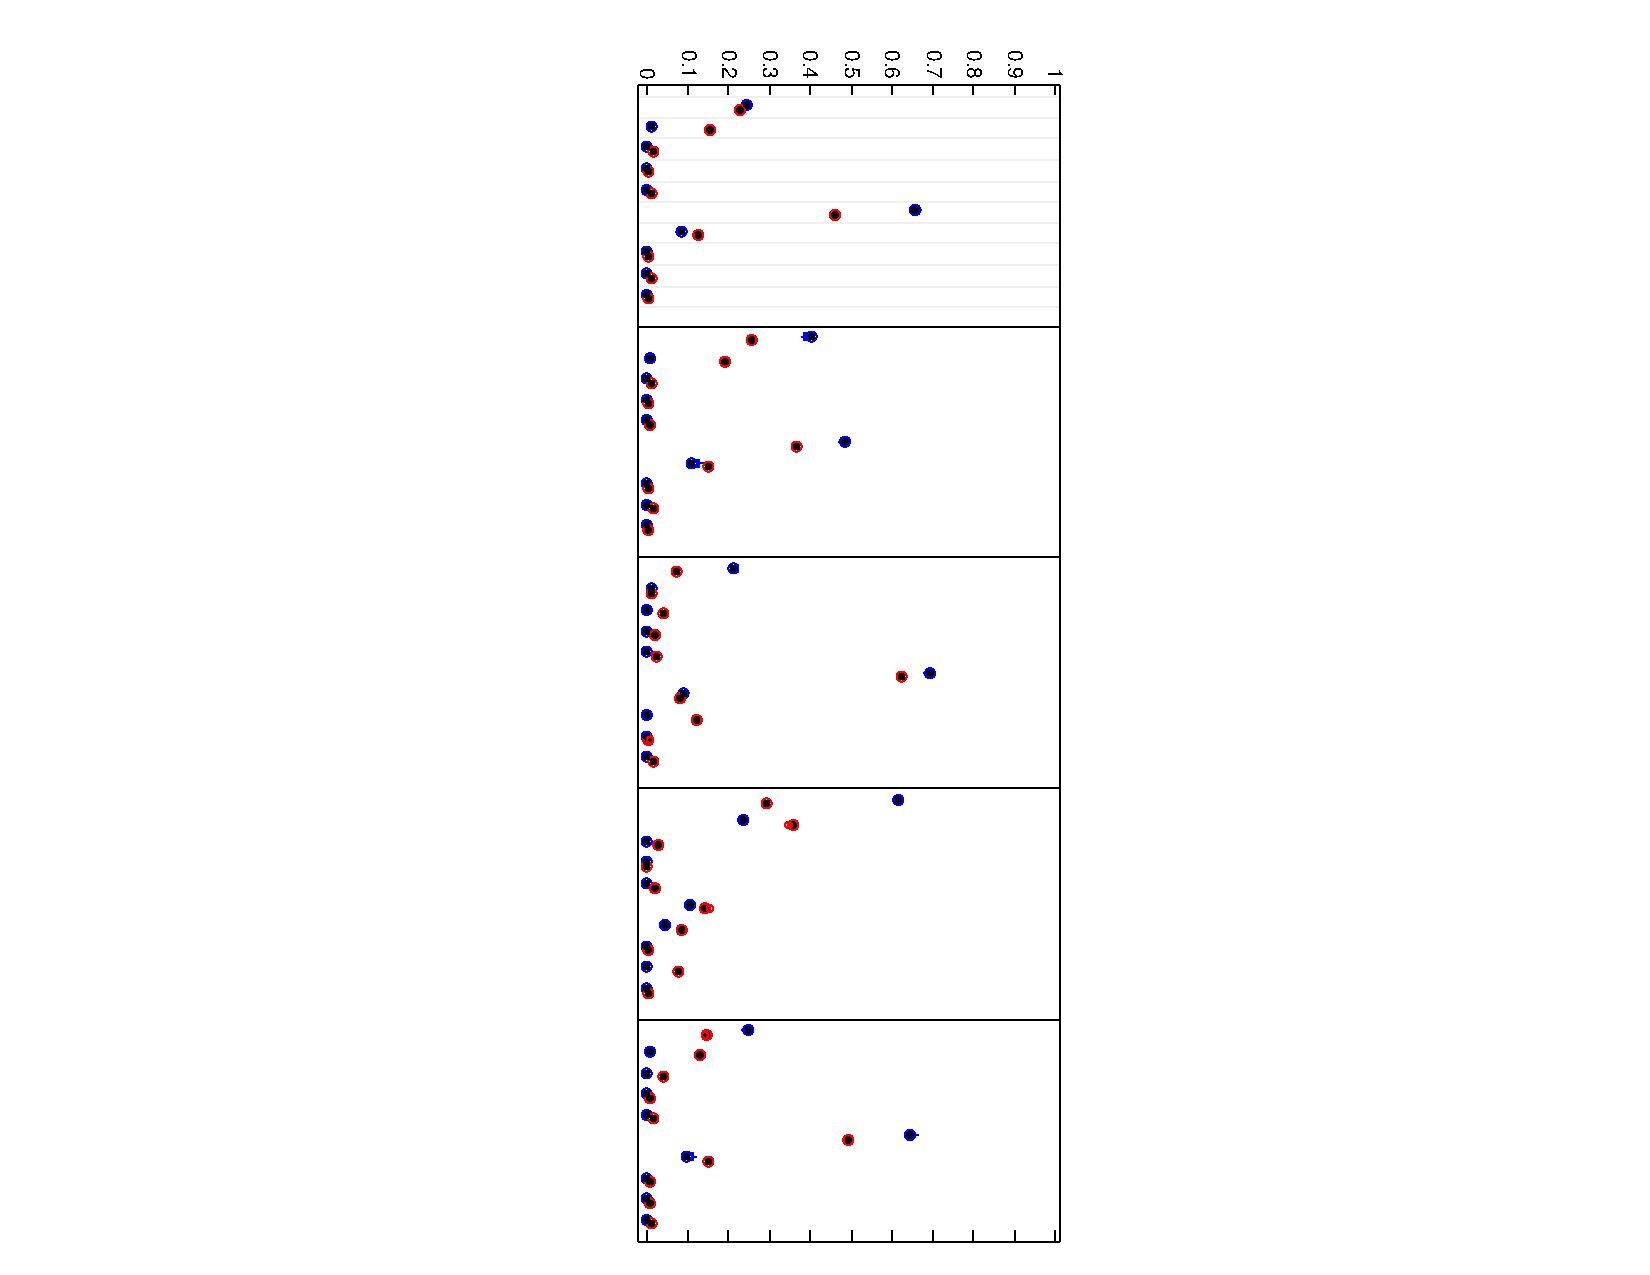
\includegraphics[trim = 305 14 277 20, clip,angle=90,width=\textwidth]{cooccurrenceMatrixB.pdf}};

\draw[] (imgNode.north west) +(18pt,4pt) node[nameSt, draw=fibroGlandColor, fill=fibroGlandColor,label=right:Fibro-glandular] (fibroGlandName) {} ;
\draw[] node[nameSt, draw=fatColor, fill=fatColor,right=of fibroGlandName,label=right:Adipose tissue] (fatName) {} ;
\draw[] node[nameSt, draw=skinColor, fill=skinColor,right=of fatName,label=right:Skin layers] (skinName) {} ;
\draw[] node[nameSt, draw=lesionColor, fill=lesionColor,right=of skinName,label=right:lesion] (lesionName) {} ;
\draw[] node[nameSt, draw=boundaryColor, fill=boundaryColor,right=of lesionName,label=right:Boundary] (boundaryName) {} ;

\end{tiny}




%\draw[] node[nameSt,draw=Gcolor, fill=Gcolor, below=of FAname,label=right:Ganglion] (Gname) {}; 
%\draw[] node[nameSt,draw=Hcolor, fill=Hcolor, below=of Gname,label=right:Harmatoma] (Hname) {}; 
%\draw[] node[nameSt,draw=CDIcolor, fill=CDIcolor, below=of Hname,label=right:Ductal Infiltrating Carcinoma] (CDIname) {}; 
%\draw[] node[nameSt,draw=CIDcolor, fill=CIDcolor, below=of CDIname,label=right:Intra-Ductal Carcinoma] (CIDname) {}; 
%\draw[] node[nameSt,draw=CLIcolor, fill=CLIcolor, below=of CIDname,label=right:Infiltrating Lobular Carcinoma] (CLIname) {}; 
%\draw[] node[nameSt,draw=Othercolor, fill=Othercolor, below=of CLIname,label=right:Other Pathologies] (Othername) {}; 



%\tikzset{nameSt/.style=
%{anchor=north west,rectangle,
%node distance=10pt,
%minimum width=8pt,minimum height=8pt,
%inner sep=0,
%}}
%\begin{tiny}
%
%\draw[] (imgNode.north east) +(5pt,0) node[nameSt, label=below:Dictionary] (dictionary) {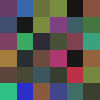
\includegraphics[width=.10\textwidth,]{fakeDict.png}} ;
%\draw[] (dictionary.north east) +(5pt,0) node[nameSt, label=below:(1)] (BoFi) {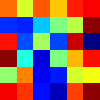
\includegraphics[width=.10\textwidth,]{BoF/desc01.png}} ;
%\draw[] (BoFi.north east) +(5pt,0) node[nameSt, label=below:(2)] (BoFii) {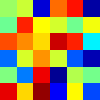
\includegraphics[width=.10\textwidth,]{BoF/desc02.png}} ;
%
%\node[nameSt, below=of dictionary, label=below:(3)] (BoFiii) {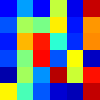
\includegraphics[width=.10\textwidth,]{BoF/desc03.png}} ;
%\node[nameSt, below=of BoFi, label=below:(4)] (BoFiv) {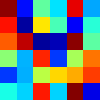
\includegraphics[width=.10\textwidth,]{BoF/desc04.png}} ;
%\node[nameSt, below=of BoFii, label=below:(5)] (BoFv) {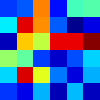
\includegraphics[width=.10\textwidth,]{BoF/desc05.png}} ;
%
%\node[nameSt, below=of BoFiii, label=below:(6)] (BoFvi) {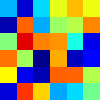
\includegraphics[width=.10\textwidth,]{BoF/desc06.png}} ;
%\node[nameSt, below=of BoFiv, label=below:(7)] (BoFvii) {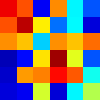
\includegraphics[width=.10\textwidth,]{BoF/desc07.png}} ;
%\node[nameSt, below=of BoFv, label=below:(8)] (BoFviii) {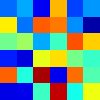
\includegraphics[width=.10\textwidth,]{BoF/desc08.png}} ;
%
%\end{tiny}

\end{tikzpicture}

\end{document}